\documentclass[10pt]{IEEEtran}

\usepackage[utf8x]{inputenc}
\usepackage[L7x]{fontenc}
\usepackage[lithuanian]{babel}
\usepackage{listings}
\usepackage{graphicx}
\usepackage{epstopdf}


\lstset{
    basicstyle=\footnotesize,
    language=Java,
    morekeywords={String,each,in,Iterator}
}

\author{Maksim Norkin\\ \texttt{maksim.norkin@ieee.org}}
\title{Modernios informacinės sistemos\\Dalis 1}

\begin{document}

    \maketitle

    \section{Laboratorinis darbas nr 1.\\Dalykinės srities pasirinkimas}

        \subsection{Užduotis}

            Dalykinę sritį aprašyti žodžiais ir pavaizduoti paveikslėlyje. Būtina bendrai aprašyti vykstančius verslo procesus. Ta pati pasirinktoji dalykinė sritis turi būti nagrinėjama visuose  tolimesniuose darbuose. 

            Reikia pateikti pasirinktos dalykinės srities aprašymą. Aprašymas turi būti tekstinis ir iliustruotas vaizdžiuoju paveikslėliu. Aprašymui sudaryti turi būti naudojami dalykinės srities  terminai. Aprašymas turi atspindėti pagrindinius dalykinės srities aktorius, procesus bei įmonės veiklą įtakojančius išorinius agentus. Aiškiai turi būti išryškinta probleminė sritis, kuri parodo, kodėl yra svarbu nagrinėti pasirinktą dalykinę sritį. 

            Taip pat gali būti vaizduojami informaciniai srautai, materialiniai srautai, sistemos veiklą  kontroliuojantys elementai, dalyvių požiūriai ir emocijos, konfliktinės situacijos. Turi būti pateikta vaizdžiojo paveikslėlio specifikacija.

        \subsection{Įvadas}

            Dalykinė sritis pasirinkimas padaromas automobilių stovėjimą teikiančios įmonės naudai. Padarius šios srities analizę, nuspręsta, kad šioje srityje galima darbą optimizuoti galinio kliento naudai.

        \subsection{Analizė}

            Iškeliama problema yra randama kiekvienos dienos situacijoje, kuomet tik važiuojame į bet kokio pobūdžio susitikimą ir reikia automobilį palikti stovėjimo aikštelėje.

            Struktūrinė automobilių stovėjimo paslaugų teikimo įmonė schema pavaizduota \ref{fig:struktur2a} pav. Jos sudarančių struktūrinių vienetų funkcijos ir ryšiai yra pateikti \ref{table:struktura} lentelėje. 

            Vienas iš problematiškiausių mazgų, yra ryšys tarp kliento ir terminalo. Jam užtikrinti reikalingas patikimas ryšys tarp banko, telekomunikacijų bendrovės, techninės priežiūros specialisto ir pavedimų posistemės vientiso veikimo. Esamą posistemę būtina suprastinti, kadangi neveikiant vienam iš posistemės mazgų -- griūna visos posistemės darbas.

            \begin{figure*}[t]
                \centering
                \includegraphics[width=540px]{figures/struktura.eps}
                \label{fig:struktur2a}
                \caption{Dalykinės srities struktūra.}
            \end{figure*}

            \begin{table*}[t]
                \centering
                \renewcommand{\arraystretch}{1.3}
                \caption{Dalykinės stuktūros paaiškinimas}
                \label{table:struktura}
                \begin{tabular}{|c|p{5cm}|p{5cm}|} \hline 
                    \textbf{Schemos objektas} & \textbf{Objekto aprašymas, funkcijos} & \textbf{Ryšiai su kitais objektais} \\ \hline

                    Direktorius & 
                    \begin{itemize} 
                        \item Darbo našumo gerinimas 
                        \item Darbo metodikos prižiūrėtojas 
                        \item Terminalų plėtra
                    \end{itemize} & 
                    \begin{itemize}
                        \item Leidimų išdavimo derinimas su savivaldybe 
                        \item Projektų derinimas su architektu 
                    \end{itemize}\\ \hline

                    Architektas & 
                    \begin{itemize}
                        \item Projektų terminų derinimas
                        \item Darbų paskirstymas
                        \item Darbo metodikos tiesioginė priežiūra 
                    \end{itemize} & 
                    \begin{itemize}
                        \item Darbo paskirstymas sistemų inžinieriui
                        \item Sistemos priežiūros darbai su administratoriumi
                    \end{itemize} \\ \hline

                    Administratorius &
                    \begin{itemize} 
                        \item Serverių priežiūra
                        \item Pavedimų saugumo užtikrinimas
                        \item Bankinės sistemos diegimas
                    \end{itemize} &
                    \begin{itemize}
                        \item Atnaujinimų priėmimas iš sistemų inžinieriaus
                        \item Atnaujinimų įgyvendinimas serveryje
                    \end{itemize} \\ \hline

                    Sistemų inžinierius &
                    \begin{itemize} 
                    \item Sprendimų įgyvendinimas
                    \item Optimaliausių sprendimų taikymas
                    \end{itemize}& 
                    \begin{itemize}
                    \item Darbų derinimas su architektu
                    \item Darbų koordinavimas su administratoriumi
                    \item Atnaujinimo parengimas administratoriui
                    \item Bankinių protokolų įgyvendinimas
                    \end{itemize}\\ \hline

                    Techninės priežiūros inžinierius &
                    \begin{itemize}
                    \item Terminalų priežiūra
                    \end{itemize} & 
                    \begin{itemize}
                    \item Darbų derinimas su telekomunikacijų bendrovėmis
                    \item Ryšio užtikrinimas su terminalu
                    \item Administratoriaus pagalba
                    \end{itemize}\\ \hline

                    Klientas &
                    \begin{itemize} 
                    \item Paslaugų naudojimas
                    \item Laiko ribų įsipareigojimas
                    \end{itemize}& 
                    \begin{itemize}
                    \item Kreipimas į terminalą
                    \item Apmokėjimo patvirtinimo gavimas
                    \end{itemize}\\ \hline
                \end{tabular}
            \end{table*}

        \subsection{Išvados}

            Laboratorinio darbo metu buvo išnagrinėta dalykinė sritis ir pažymėta jos pagrindinė probleminė sritis. Pateikta dalykinės srities struktūros schema, bei jos funkcinis ir ryšių aprašymas. Būtina optimizuoti ir suprastinti kliento naudojimosi terminalu sistema ir ją suprastinti, kadangi keturių mazgų sistema gali būti labai nepatikima.

    \section{Laboratorinis darbas nr. 2}

        \subsection{Užduotis}

            Verslo sistemos tikslų modeliavimas. Apibrėžti strateginį tikslą ir operacinius tikslus, nurodyti jų hierarchinius ryšius. Tikslas nurodo siekiamą būseną. Tikslai gali būti kiekybiniai (pamatuojami) ar kokybiniai.

            Kiekvienam kiekybiniam tikslui nurodyti:

            \begin{itemize}
                \item Koks jo matavimo vienetas
                \item Kokia esama vertė
                \item Per kokį laikotarpį reikia nurodytą vertę pasiekti
            \end{itemize}    

            Žemiausio lygmens operacinio lygmens tikslams nurodyti:

            \begin{itemize}
                \item Problemą(-as), kurios trukdo tą tikslą įgyvendinti
                \item Problemos priežastį
                \item Veiksmą, kuris nurodo problemos sprendimo strategiją
                \item Uždavinius, kurių įgyvendinimas padeda išspręsti problemą
            \end{itemize}

            Tikslų ir/ar problemų, priežasčių, veiksmų ir uždavinių hierarchinę struktūrą galima atvaizduoti, naudojant UML klasių diagramą.

        \subsection{Įvadas}

        \subsection{Analizė}

        \subsection{Išvados}

    \section{Laboratorinis darbas nr. 3}

        \subsection{Užduotis}

            Verslo sistemos organizacinės struktūros modeliavimas. Šiame darbe reikia aprašyti įmonės organizacinę struktūrą. Aprašoma tik analizuojama įmonės dalis. Analizuojamos įmonės ribos yra apibrėžtos vaizdžiajame paveikslėlyje. Organizacinę struktūrą galima modeliuoti:
            
            \begin{itemize}
                \item Pagal įmonės departamentus, jų skyrius ir poskyrius
                \item Pagal darbuotojų vaidmenis, kitais žodžiais sakant pagal darbuotojų užimamas pareigas, hierarchinius ryšius
            \end{itemize}

            Kurį būdą geriau pasirinkti priklauso nuo jūsų pasirinktos analizuojamos srities. Grafiškai organizacinę struktūrą galima atvaizduoti, naudojant UML klasių diagramą.

        \subsection{Įvadas}

        \subsection{Analizė}

        \subsection{Išvados}

    \section{Laboratorinis darbas nr. 4}

        \subsection{Užduotis}

            Verslo sistemos procesų modeliavimas. Aprašyti bent 3 procesus. Pateikti procesų naudojamus išteklius, proceso veikimo rezultatus, kokius tikslus įgyvendina procesas., kas jį valdo ir t.t. Paprastai tam naudojama klasių arba objektų diagrama. Kiekvienam procesui yra pateikiama veiklos ir/arba sekų diagrama, kurioje detaliai parodyta, kaip vykdomas procesas, kas jį vykdo.

        \subsection{Įvadas}

        \subsection{Analizė}

        \subsection{Išvados}

    \section{Laboratorinis darbas nr. 5}

        \subsection{Užduotis}

            Pateikiamos verslo sistemos užduotys. Kiekvienas užduoties vykdymas parodomas naudojant veiklos ir/arba sekų ir/arba ansamblių diagramas. Kiekvieną užduotį specifikuoti naudojant:

            \begin{itemize}
                \item Užduotis pavadinimą
                \item Tikslą
                \item Sėkmės veiksnius
                \item Sėkmės vertinimo kriterijus
                \item Ypatingas situacijas
                \item Variantus
            \end{itemize}

        \subsection{Įvadas}

        \subsection{Analizė}

        \subsection{Išvados}

\end{document}